\chapter{Quelles sont les sources d'informations exploitables?}


Le sujet de départ de l'étude, qui est mené actuellement à l'ENSTA Bretagne, est de proposer des méthodes d'identification et de caractérisation de la thrombose et du thrombose veineuse profonde ou DVT. Cette étude est menée en partenariat avec plusieurs medecins du CHRU de Brest, M. Bressollette et M. Moittier qui fournissent actuellement la majorité des images qui sont utilisées pour cette étude. Dans un premier temps, nous nous sommes intéressés aux différents types d'image que nous pouvions avoir accès. 


\section{Elastométrie}

L'élastométrie est une méthode d'acquisition d'image médicale non invasive et très pratique. En effet, très facile à mettre en œuvre et peu couteuse en temps et en argent. Cette méthode consiste à créer une représentation d'une zone du corps à partir de l'élasticité du tissu biologique \cite{ophir1991elastography}.

\begin{figure}[H]
\centering
    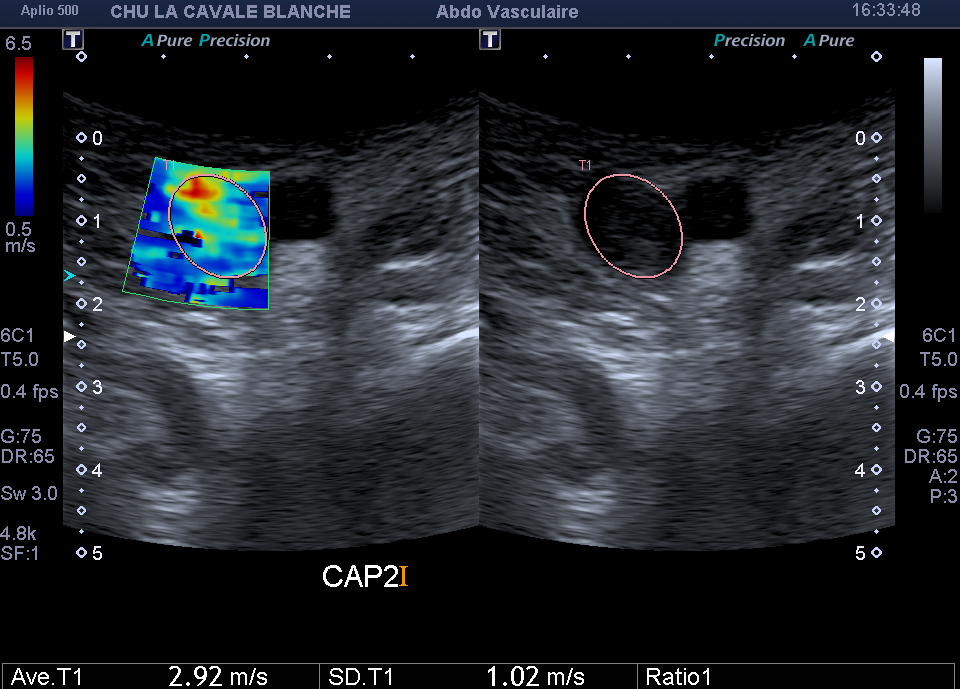
\includegraphics[scale=0.3,angle=0]{Images/ExempleElastometrie.png}
    \caption{Exemple d'image d'élastometrie.}
    \label{fig:ExempleElastometrie}
\end{figure}

Cette méthode présente plusieurs particularités pour cette étude:

\begin{itemize}
\item Elle est très facile à utiliser et se fait en un temps très faible. 
\item C'est une méthode qui n'est pas invasive.
\item Bien que la mise en œuvre soit facile, les images obtenues sont de médiocre qualité en terme de résolution.
\end{itemize}

Néanmoins, il y a un problème à cette méthode. Il est nécessaire de définir un protocole unique à tous les patients pour faire en sorte que les images obtenues par ce procédé soient comparables.

 
\section{Échographie}

L'échographie est une technique d'imagerie qui consiste à utiliser des ondes ultrasons. En fonction des propriétés du milieu, certains tissus ou partie du corps apparaitront en noir, gris ou blanc. 

\begin{figure}[H]
\centering
    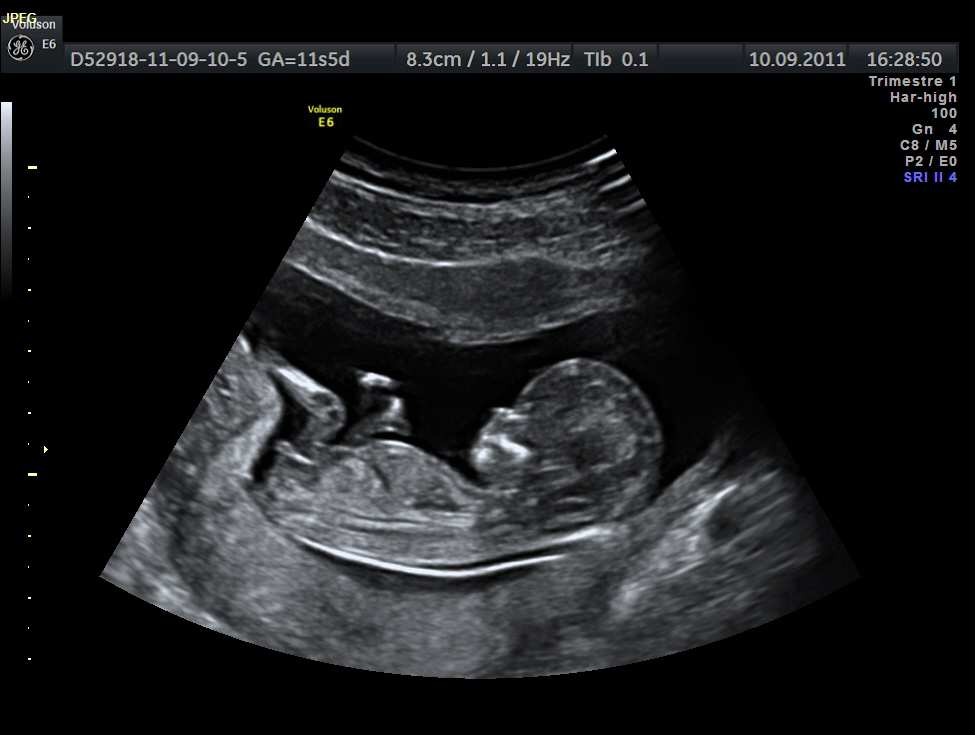
\includegraphics[scale=0.6,angle=0]{Images/Echographie-profil.jpg}
    \caption{Exemple d'image échographique pour l'obstétrie.}
    \label{fig:Echographie}
\end{figure}

Cette méthode présente les mêmes avantages que l'élastométrie. Elle est peu chère, facile à mettre en œuvre et non invasive pour le patient. Néanmoins, elle présente également des images de très faible qualité en terme de résolution.


\section{Computed tomography angiography / Angiographie}

L'angiographie est une technique d'imagerie qui est invasive. Bien qu'elle présente plusieurs intérêts, notamment car elle consiste à faire une imagerie des vaisseaux sanguins par rayon X (veines ou artères), il y a plusieurs effets secondaires (vomissement, vertiges, nausées, réactions allergiques, saignement important...) ou contre-indications (grossesse, tension artérielle trop basse...). Cette piste ne sera pas étudiée ici.

\begin{figure}[H]
\centering
    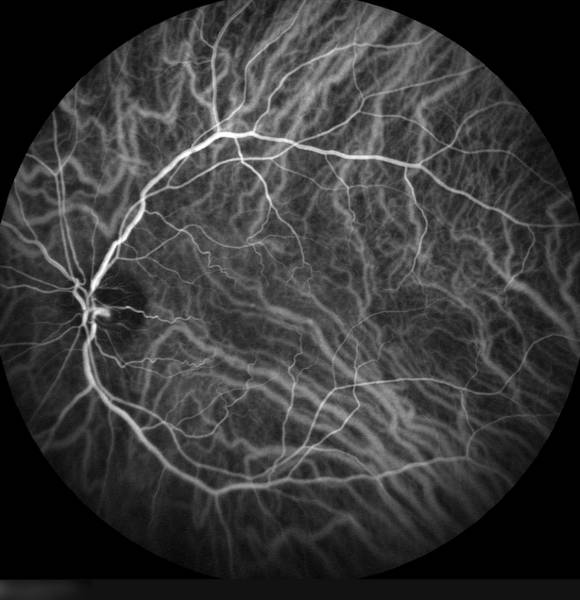
\includegraphics[scale=0.4,angle=0]{Images/m_1407858437.jpg}
    \caption{Exemple d'angiographie pour l'œil.}
    \label{fig:m_1407858437}
\end{figure}

\section{Scanner}

Le scanner est un outil qui propose de reconstituer des images des tissus par ordinateur à partir des différences d'absorption des rayons X. Ce procédé permet d'obtenir des coupes du corps du patient très rapidement et présente certains avantages et inconvénients. C'est une méthode qui permet d'obtenir très rapidement des images médicales exploitable pour faire un diagnostic. Néanmoins, c'est un procédé qui impose l'utilisation de rayon X donc irradiant. C'est donc un procédé invasif.


\begin{figure}[H]
\centering
    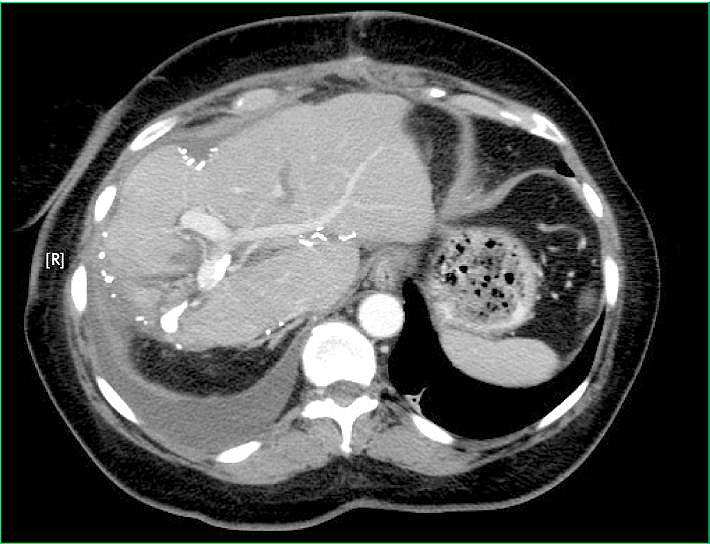
\includegraphics[scale=0.4,angle=0]{Images/Scanner.jpg}
    \caption{Exemple d'image issue d'un scanner.}
    \label{fig:m_1407858437}
\end{figure}

\section{IRM}

L'IRM ou l'imagerie par résonance magnétique sera ici la source d'image médicale qui sera étudiée. Elle produit des images avec une haute résolution et présent un énorme avantage pour nous. C'est un procédé entièrement non invasif et, à la différence du scanner, elle ne nécessite aucun produit irradiant.

\begin{figure}[H]
\centering
    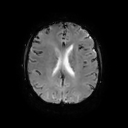
\includegraphics[scale=2,angle=0]{Images/Im7.png}
    \caption{Exemple d'image IRM.}
    \label{fig:m_1407858437}
\end{figure}

Le principe de base de l'IRM est de faire une imagerie des atomes d'hydrogène présent dans le tissu que nous souhaitons étudier. Nous considérons ici que le noyau de l'atome d'hydrogène qui est juste un proton qui tourne sur lui-même. L'idée est d'utiliser un puissant aimant qui va générer un champs et une onde radio excitatrice de fréquence identique à la fréquence de rotation des protons. Ceci a pour conséquence que tous les protons tournent dans un même axe qui est légèrement différent de l'axe du champs de l'aimant et qu'ils soient en phase. Ce léger écart dans l'orientation de l'axe est dû à l'excitation par l'onde radio.

A partir de ce point, on coupe l'onde excitatrice et deux phénomènes se présentent:

\begin{itemize}
\item Les protons vont revenir à leur état chaotique de départ et vont tous se déphaser,
\item Les protons vont tous s'orienter par rapport à l'axe du champs de l'aimant.
\end{itemize}

Ce changement d'état se traduit par la diffusion d'un signal qui est capté et permet la réalisation de la cartographie des protons et donc de notre image IRM. On peut paramétrer la machine pour mesurer deux paramètres:

\begin{itemize}
\item Soit on mesure le temps que mettent les protons pour se remettre dans l'axe de l'aimant ce qui est appelé temps de relaxation T1 ou pondération T1.
\item Soit on mesure le temps que mettent les protons pour se désynchroniser ce qui est appelé temps de relaxation T2 ou pondération T2.
\end{itemize}


\chapter{Premier sujet: Caractérisation de la thrombose par les IRM}


Pendant la durée du stage, nous étions deux à travailler sur la problématique de la détection et de la caractérisation de la thrombose. Thibaud Berthomier qui est actuellement en thèse à l'ENSTA Bretagne a pu récupérer de la part du CHRU plusieurs images de caillot sanguin. L'étude qu'il mène se concentre sur les caillots situés au niveau de la cuisse. Je devais, pour ma part, explorer une autre piste qui consistait à utiliser des images IRM. Je devais également utiliser le résultat d'une thèse pour voir si la méthode qui y est dévellopée pouvait être utilisée \cite{tartare2014contribution}, \cite{tartare2014spectral}. Il nous a fallu donc dans un premier temps faire un état de l'art sur les éléments développés dans cette thèse et sur le thrombose veineuse profonde (DVT).


\section{Première piste, utilisation des IRM de perfusion.}

Le principe de l'IRM de perfusion est d'injecter un produit de contraste, ici le galonium, qui est visible par IRM et de voir comment ce produit se diffuse au cours du temps dans les différentes zones du corps. A terme, nous obtenons un ensemble d'image traduisant l'évolution de la concentration du produit dans la zone étudiée au cours du temps. A partir de ces images, nous pouvons déterminer la courbe d'intensité au cours du temps de chaque pixel de l'IRM. L'idée est donc de voir le comportement d'une zone du corps avant, pendant et après injection du produit de contraste et de voir si on peut caractériser ainsi une zone en particulier.

Dans un premier temps, nous souhaitions utiliser la méthodologie mise au point dans la thèse \cite{tartare2014contribution}. Cette dernière propose deux outils pour l'aide au diagnostic. Le premier est l'établissement de carte de paramètre pharmacocinétique. Le second est l'utilisation d'algorithme de classification non supervisé pour réaliser des clusters à partir différentes courbes d'intensité obtenues afin d'isoler les courbes présentant le même comportement entre elles. Ainsi, on obtient une nouvelle carte segmentée qui indique les régions qui présentent les même caractéristiques.

\begin{figure}[H]
\centering
    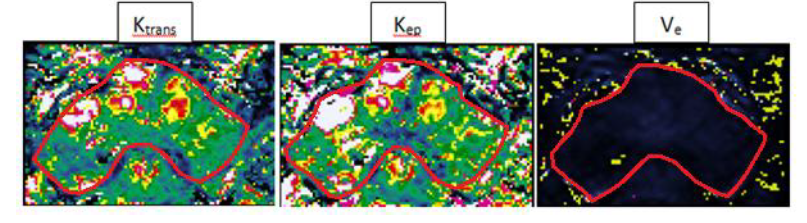
\includegraphics[scale=0.6,angle=0]{Images/CatreDeParametresPharmacocinetique.png}
    \caption{Cartes de parametre pharmacocinetique $K_p, K_{trans}$ et $V_e$ de la prostate.}
    \label{fig:CarteDeParametresPharmacocinetique}
\end{figure}

La figure qui suit montre la méthodologie appliquée ici \ref{fig:Classif}.
 
\begin{figure}[H]
\centering
    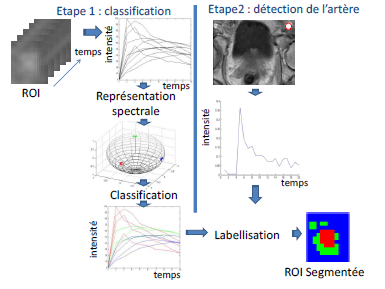
\includegraphics[scale=1,angle=0]{Images/Classif.png}
    \caption{Méthodologie suivie pour la classification.}
    \label{fig:Classif}
\end{figure}

L'idée est d'avoir au final des images qui segmentent directement les tissus sains et les tissus pathologiques.

\section{Qu'est ce que la thrombose veineuse profonde}

On appelle thrombose le fait qu'un caillot sanguin ou thrombus se développe à l'intérieur d'un vaisseau sanguin. Il peut être soit artériel, soit veineux. Dans les deux cas, ce caillot peut obstruer le vaisseau et donc empêcher la circulation du sang.

\begin{figure}[H]
\centering
    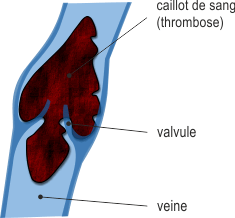
\includegraphics[scale=2,angle=0]{Images/phleb1.png}
    \caption{Exemple illustrant la thrombose.}
    \label{fig:phleb1}
\end{figure}

La phlébite est un cas de thrombose veineuse pour une veine profonde et est consécutif à l'inflammation de la veine et au risque de déplacement du caillot. D'où le terme de thrombose veineuse profonde DVT (deep venous thrombose).

Parmi les principales causes, nous pouvons énumérer:


\begin{itemize}
\item Une lésion dans une veine qui entraine une coagulation au niveau du tissu sanguin (blessure...),
\item Certains paramètres génétiques qui peuvent favoriser le processus de thrombose,
\item Les périodes prolongées dans une même position (alitement, accouchement, voyage long en avion...),
\item Des précédentes expériences traumatisantes pour le corps (cancer, opération...),
\item Influence de certaines substances sur la paroi des artères (tabac, médicaments...), 
\item Facteurs favorisant la formation de thrombus (obésité, diabète, hypercholestérolémie...). 
\end{itemize}

Une fois le caillot formé, il peut se produire différents phénomènes:

\begin{itemize}
\item Il peut de lui même se désagréger et disparaitre naturellement,
\item Il peut se calcifier ou changer de structure se qui peut amener à la formation de pelote fibreuse,
\item Il peut se détacher et atteindre un des vaisseaux pulmonaires. Ceci se traduit par une embolie pulmonaire qui s'avère très dangereux.
\end{itemize}

Dans tous les cas, la présence de ce caillot dans le système circulatoire sanguin d'un patient peut mener à des perturbations graves du flux sanguin avec l'apparition d'œdème ou d'ulcère pour la zone inférieure du corps que nous allons étudier.

\section{Problème rencontré vis à vis des IRM de thrombus.}

Les premières semaines du stage ont donc consisté à tenter de récupérer des images IRM de thrombus afin de voir ce qui était possible de faire. Très rapidement, plusieurs problèmes se sont présentés:

\begin{itemize}
\item Le fait d'utiliser des IRM pour des caillots sanguins est encore très récent et nécessite la création de nouveaux protocoles qui doivent être validés par des comités d'éthique. Cette démarche prend beaucoup de temps et cette utilisation des IRM reste encore au niveau de la recherche expérimentale.
\item Il n'y a pour l'instant aucune image IRM de caillot situé au niveau de la cuisse, caillot qui est pour l'instant principalement étudié.
\item Pour les thrombus cérébraux, il existe des IRM mais plusieurs problèmes se sont rapidement manifestés. La signature IRM du caillot change assez rapidement en fonction de son âge. De plus, sa composition et sa position ont un lourd impact sur comment il sera vu sur l'IRM.
\end{itemize}

Au final, si nous devions poursuivre sur cette voie, nous aurions dû nous concentrer sur les thromboses cérébraux. De plus, après plusieurs discussions avec les médecins du CHRU, cela aurait nécessité un travail qui n'était pas réalisable en 6 mois.

\chapter{Changement de sujet: Réalisation d'un programme d'aide au diagnostic pour les pathologies cérébrales.}


Après une période d'investigation qui a démontré que le premier objectif était irréalisable dans le temps imparti, les médecins du CHRU m'ont proposé de réaliser un programme d'aide au diagnostic pour les pathologies cérébrales. Ces derniers étaient justement spécialisés sur cette partie du corps humain et pouvaient me fournir les images nécessaires pour que je puisse travailler. 
De plus, j'ai pu prendre contact avec les personnes qui ont encadré la thèse sur laquelle je m'appuyais pour récupérer leurs données expérimentales et simulées. J'ai donc pu déjà profiter de leur expertise et d'autre part récupérer plusieurs données simulées de prostate présentant des tumeurs et plusieurs IRM de perfusion de prostate présentant cette pathologie.

\begin{figure}[H]
\centering
    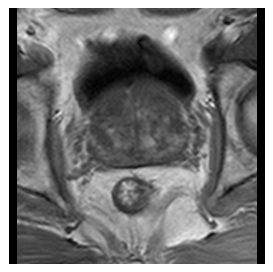
\includegraphics[scale=1,angle=0]{Images/ProstateImage.png}
    \caption{Image IRM de la prostate.}
    \label{fig:ProstateImage}
\end{figure}

Au final, j'ai pu récupérer avec le CHRU les IRM de perfusion de 13 patients présentant des pathologies assez visibles pour que je puisse tester mes algorithmes. Parmi les pathologies qui ont été recensées, il y a plusieurs formes de cancer et des œdèmes assez significatifs. Le travail qui va suivre a donc pour but de voir quelles sont les pathologies qui peuvent être identifiées par cette méthode, généraliser et proposer des améliorations au niveau de la chaine de traitement et donc réaliser un programme d'aide au diagnostic pour ces pathologies.




